% !TEX program = lualatex

% Template for the submission to:
%   Econometrica   [ecta]
%
%%%%%%%%%%%%%%%%%%%%%%%%%%%%%%%%%%%%%%%%%%%%%%
%% In this template, the places where you   %%
%% need to fill in your information are     %%
%% indicated by '???'.                      %%
%%                                          %%
%% Please do not use \input{...} to include %%
%% other tex files. Submit your LaTeX       %%
%% manuscript as one .tex document.         %%
%%%%%%%%%%%%%%%%%%%%%%%%%%%%%%%%%%%%%%%%%%%%%%

% use option [draft] for initial submission
%            [final] for the prepublication
\RequirePackage{fontspec}
\def\econselectedclass{econsocart}
\def\econjournalclass{econsocart}
\ifx\econselectedclass\econjournalclass
\documentclass[ecta,nameyear,draft]{econsocart}
\else
\documentclass[]{econsocart}
\fi
%
%

\RequirePackage[colorlinks,citecolor=blue,linkcolor=blue,urlcolor=blue,pagebackref]{hyperref}

% 日本語対応のためのパッケージ
% \usepackage{luatexja}
\usepackage{luatexja-fontspec}
\usepackage{float}
\usepackage{booktabs}
\usepackage{longtable}
\newcommand{\hiddenlabel}[1]{\refstepcounter{equation}\label{#1}}
\newcommand{\hiddenfiglabel}[1]{\refstepcounter{figure}\label{#1}}
\newcommand{\hiddentablabel}[1]{\refstepcounter{table}\label{#1}}

\let\econbibstyle\bibliographystyle
\renewcommand{\bibliographystyle}[1]{}
\makeatletter
\@ifundefined{KOMAClassName}{% if non-KOMA class
  \IfFileExists{parskip.sty}{%
    \usepackage{parskip}
  }{% else
    \setlength{\parindent}{0pt}
    \setlength{\parskip}{6pt plus 2pt minus 1pt}}
}{% if KOMA class
  \KOMAoptions{parskip=half}}
\makeatother
% Make \paragraph and \subparagraph free-standing
\makeatletter
\ifx\paragraph\undefined\else
  \let\oldparagraph\paragraph
  \renewcommand{\paragraph}{
    \@ifstar
      \xxxParagraphStar
      \xxxParagraphNoStar
  }
  \newcommand{\xxxParagraphStar}[1]{\oldparagraph*{#1}\mbox{}}
  \newcommand{\xxxParagraphNoStar}[1]{\oldparagraph{#1}\mbox{}}
\fi
\ifx\subparagraph\undefined\else
  \let\oldsubparagraph\subparagraph
  \renewcommand{\subparagraph}{
    \@ifstar
      \xxxSubParagraphStar
      \xxxSubParagraphNoStar
  }
  \newcommand{\xxxSubParagraphStar}[1]{\oldsubparagraph*{#1}\mbox{}}
  \newcommand{\xxxSubParagraphNoStar}[1]{\oldsubparagraph{#1}\mbox{}}
\fi
\makeatother
\usepackage{longtable,booktabs,array}
\newcounter{none} % for unnumbered tables
\usepackage{calc} % for calculating minipage widths
% Correct order of tables after \paragraph or \subparagraph
\usepackage{etoolbox}
\makeatletter
\patchcmd\longtable{\par}{\if@noskipsec\mbox{}\fi\par}{}{}
\makeatother
% Allow footnotes in longtable head/foot
\IfFileExists{footnotehyper.sty}{\usepackage{footnotehyper}}{\usepackage{footnote}}
\makesavenoteenv{longtable}
\usepackage{graphicx}
\makeatletter
\newsavebox\pandoc@box
\newcommand*\pandocbounded[1]{% scales image to fit in text height/width
  \sbox\pandoc@box{#1}%
  \Gscale@div\@tempa{\textheight}{\dimexpr\ht\pandoc@box+\dp\pandoc@box\relax}%
  \Gscale@div\@tempb{\linewidth}{\wd\pandoc@box}%
  \ifdim\@tempb\p@<\@tempa\p@\let\@tempa\@tempb\fi% select the smaller of both
  \ifdim\@tempa\p@<\p@\scalebox{\@tempa}{\usebox\pandoc@box}%
  \else\usebox{\pandoc@box}%
  \fi%
}
% Set default figure placement to htbp
\def\fps@figure{htbp}
\makeatother
\ifLuaTeX
\usepackage[bidi=basic,shorthands=off,provide=*]{babel}
\else
\usepackage[bidi=default,shorthands=off,provide=*]{babel}
\fi
\ifLuaTeX
  \usepackage{selnolig} % disable illegal ligatures
\fi
\setlength{\emergencystretch}{3em} % prevent overfull lines
\providecommand{\tightlist}{%
  \setlength{\itemsep}{0pt}\setlength{\parskip}{0pt}}
\usepackage[]{natbib}
\bibliographystyle{ecta-fullname}

\let\bibliographystyle\econbibstyle
\babeladjust{bidi.text=off}
\makeatletter
\@ifpackageloaded{caption}{}{\usepackage{caption}}
\AtBeginDocument{%
\ifdefined\contentsname
  \renewcommand*\contentsname{目次}
\else
  \newcommand\contentsname{目次}
\fi
\ifdefined\listfigurename
  \renewcommand*\listfigurename{図一覧}
\else
  \newcommand\listfigurename{図一覧}
\fi
\ifdefined\listtablename
  \renewcommand*\listtablename{表一覧}
\else
  \newcommand\listtablename{表一覧}
\fi
\ifdefined\figurename
  \renewcommand*\figurename{図}
\else
  \newcommand\figurename{図}
\fi
\ifdefined\tablename
  \renewcommand*\tablename{表}
\else
  \newcommand\tablename{表}
\fi
}
\@ifpackageloaded{float}{}{\usepackage{float}}
\floatstyle{ruled}
\@ifundefined{c@chapter}{\newfloat{codelisting}{h}{lop}}{\newfloat{codelisting}{h}{lop}[chapter]}
\floatname{codelisting}{コード}
\newcommand*\listoflistings{\listof{codelisting}{コード一覧}}
\makeatother
\makeatletter
\makeatother
\makeatletter
\@ifpackageloaded{caption}{}{\usepackage{caption}}
\@ifpackageloaded{subcaption}{}{\usepackage{subcaption}}
\makeatother
\AtBeginEnvironment{longtable}{\def\_{\textunderscore\allowbreak}}
\newcounter{pandocauthor}
\newcommand{\pandocauthor}[1]{\stepcounter{pandocauthor}\author[id=au\arabic{pandocauthor},addressref={add1}]{\fnms{}~\snm{#1}\ead[label=e\arabic{pandocauthor}]{}}}
\ifx\econselectedclass\econjournalclass
\startlocaldefs

%%%%%%%%%%%%%%%%%%%%%%%%%%%%%%%%%%%%%%%%%%%%%%
%%                                          %%
%% Uncomment next line to change            %%
%% the type of equation numbering           %%
%%                                          %%
%%%%%%%%%%%%%%%%%%%%%%%%%%%%%%%%%%%%%%%%%%%%%%
%\numberwithin{equation}{section}
%%%%%%%%%%%%%%%%%%%%%%%%%%%%%%%%%%%%%%%%%%%%%%
%%                                          %%
%% For Assumption, Axiom, Claim, Corollary, %%
%% Lemma, Theorem, Proposition, Hypothezis, %%
%% Fact                                     %%
%% use \theoremstyle{plain}                 %%
%%                                          %%
%%%%%%%%%%%%%%%%%%%%%%%%%%%%%%%%%%%%%%%%%%%%%%
%\theoremstyle{plain}
%\newtheorem{???}{???}
%\newtheorem*{???}{???}
%\newtheorem{???}{???}[???]
%\newtheorem{???}[???]{???}
%%%%%%%%%%%%%%%%%%%%%%%%%%%%%%%%%%%%%%%%%%%%%%
%%                                          %%
%% For Definition, Example, Remark,         %%
%% Notation, Property                       %%
%% use \theoremstyle{remark}                %%
%%                                          %%
%%%%%%%%%%%%%%%%%%%%%%%%%%%%%%%%%%%%%%%%%%%%%%
%\theoremstyle{remark}
%\newtheorem{???}{???}
%\newtheorem*{???}{???}
%\newtheorem{???}{???}[???]
%\newtheorem{???}[???]{???}

%%%%%%%%%%%%%%%%%%%%%%%%%%%%%%%%%%%%%%%%%%%%%%
%% Please put your definitions here:        %%
%%%%%%%%%%%%%%%%%%%%%%%%%%%%%%%%%%%%%%%%%%%%%%


\endlocaldefs
\fi

\begin{document}

\ifx\econselectedclass\econjournalclass
\begin{frontmatter}

\title{合成経済の推定と均衡比較}
\runtitle{合成経済の推定と均衡比較}

\begin{aug}
% use \particle for den|der|de|van|von (only lc!)
% [id=?,addressref=?,corref]{\fnms{}~\snm{}\ead[label=e?]{}\thanksref{}}
%
%% e-mail is mandatory for each author
%
%%% initials in fnms (if any) with spaces
%

%%%%%%%%%%%%%%%%%%%%%%%%%%%%%%%%%%%%%%%%%%%%%%
%% Addresses                                %%
%%%%%%%%%%%%%%%%%%%%%%%%%%%%%%%%%%%%%%%%%%%%%%
\address[id=add1]{}

\support{}

%% Put support info here.  Reminder: do not thank the handling coeditor anonymously or by name
%% \support{We thank ???.}
%




\end{aug}

\end{frontmatter}
\else
\title{合成経済の推定と均衡比較}
\author{}
\date{2026-11-07}
\maketitle


\fi
%%%%%%%%%%%%%%%%%%%%%%%%%%%%%%%%%%%%%%%%%%%%%%%%%%%%%%%%%%%%%%%%%%%%%%%%%
%%%% Main text entry area:
%%%%%%%%%%%%%%%%%%%%%%%%%%%%%%%%%%%%%%%%%%%%%%%%%%%%%%%%%%%%%%%%%%%%%%%%%

\section{研究質問と採用した経済モデル}\label{data}

8つの合成経済は、それぞれの研究質問に対応する入力仕様、推定・較正、比較条件を持つ。各ケースの表図は、同じ結果
ID の推定値・政策・均衡・厚生を示す。

\begin{minipage}{\linewidth}

\section{段階的導入と効果の時間構造}\label{result-1}

政策を第3期・第5期に導入する主体について、導入後の成果がいつ変化するかを問う。対象は360主体・7期、2,520行の合成パネルである。未処置群を対照とし、共変量
x を条件とする平行トレンド、重なり、先行反応ゼロを採用する。群・時点別
ATT を did::att\_gt の二重頑健法で推定し、did::aggte
で導入からの期数別に集計した。推論は解析標準誤差、正規参照、点別95\%区間である。基準期の指定は
varying である。

\href{https://github.com/yoshimurahiroki/econ-project-mini/blob/f9093ba87cabce7bee1fdf3391656544617a8cb9/examples/research-workspace/models/did-spec.json}{入力仕様}・\href{https://github.com/yoshimurahiroki/econ-project-mini/blob/f9093ba87cabce7bee1fdf3391656544617a8cb9/examples/research-workspace/models/did-result.json}{計算結果}。

\begin{longtable}[]{@{}ll@{}}
\caption{括弧内は保存された標準誤差。単位: outcome units / 区間水準:
0.95 / 保存区間: pointwise。標本: id\_column: id, input\_rows: 2520,
observations: 360、母集団: seeded simulated units、観測単位: panel
entity、期間: simulated、単位: outcome units、推定対象: did::aggte
dynamic overall ATT、推定方法: staggered\_did、信頼区間: 0.95、N:
360、推論: confidence\_level: 0.95, interval\_type: pointwise,
overall\_interval\_type: pointwise, reference: normal,
standard\_error\_method: analytical、区間の種類: pointwise、集計:
dynamic。結果ID: specialist-did-r01。specialist-did-r01 生成元: model:
staggered\_did, specification: 079364a19e0d}\tabularnewline
\toprule\noalign{}
項目 & DR-DID \\
\midrule\noalign{}
\endfirsthead
\toprule\noalign{}
項目 & DR-DID \\
\midrule\noalign{}
\endhead
\bottomrule\noalign{}
\endlastfoot
& (1) \\
導入後の平均 ATT & 1.6588 \\
& (0.1094) \\
区間 & {[}1.4442, 1.8733{]} \\
p 値 & 6.97e-52 \\
主体数 & 360 \\
単位 & outcome units \\
\end{longtable}

\end{minipage}

\section{段階的導入と効果の時間構造の結果}\label{result-2}

導入後の平均 ATT は 1.6588、標準誤差は 0.1094、95\%区間は {[}1.4442,
1.8733{]} となる。導入期の ATT は 1.6110、翌期は 1.8491
である。導入から0--2期は2導入群、3--4期は第3期導入群を集計する。処置前の共同検定は統計量7.3359、p値
0.11917 を返した。

\begin{figure}[H]

{\centering \pandocbounded{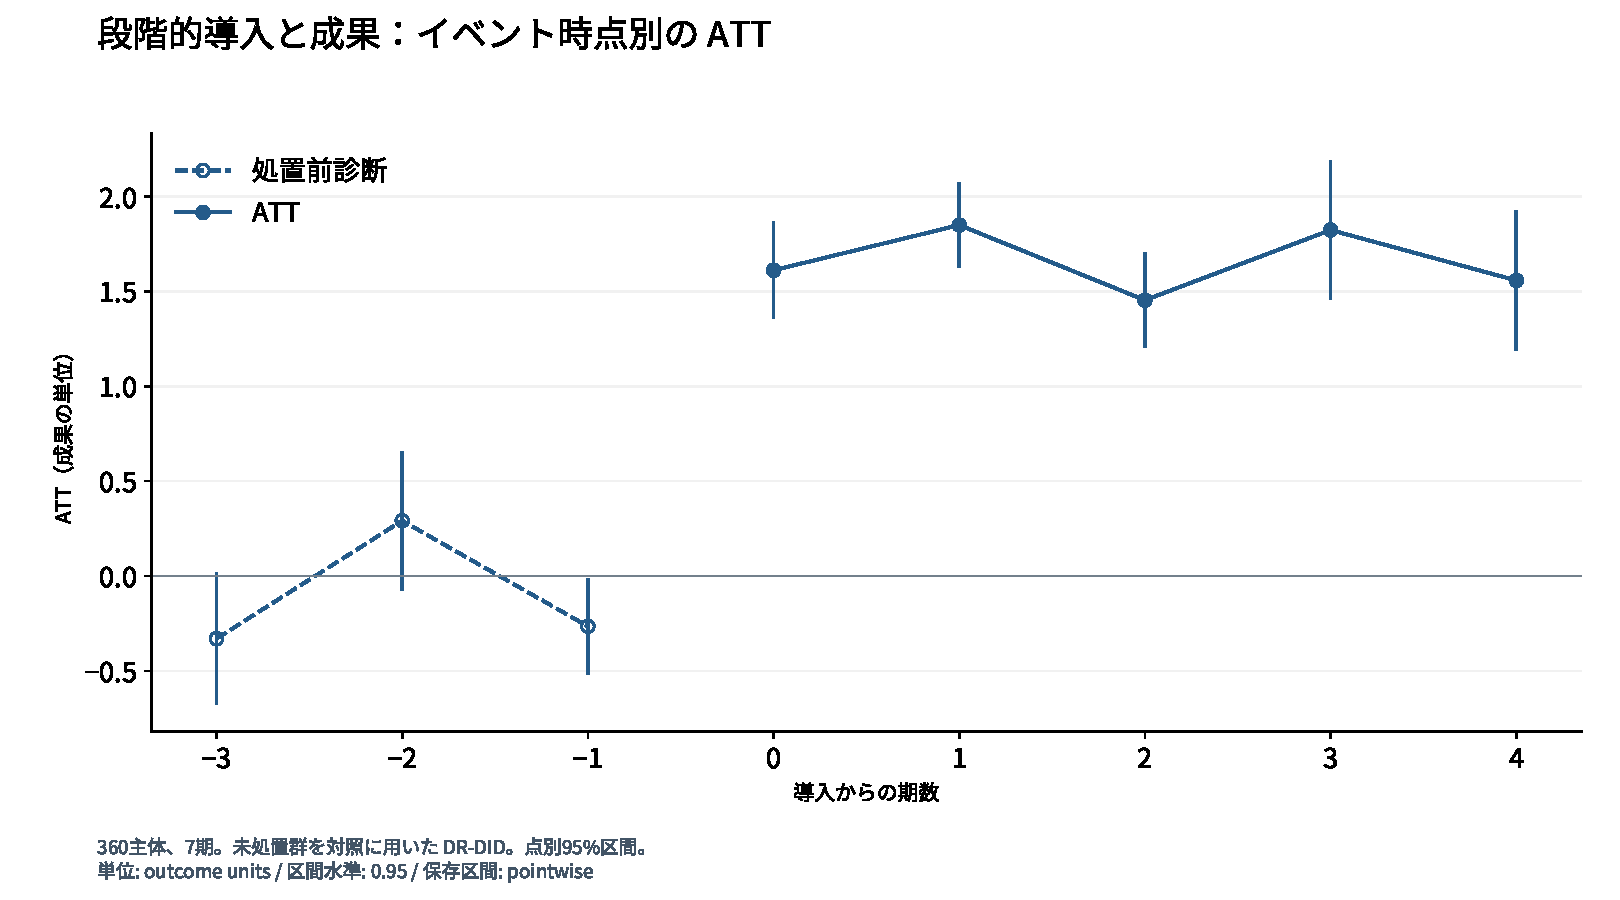
\includegraphics[keepaspectratio,alt={段階的導入と成果：イベント時点別の ATT}]{assets/exhibit-2-4.pdf}}

}

\caption{段階的導入と成果：イベント時点別の ATT.
360主体、7期。未処置群を対照に用いた DR-DID。点別95\%区間。標本:
id\_column: id, input\_rows: 2520, observations: 360、母集団: seeded
simulated units、期間: simulated、単位: outcome units、推定対象:
group-time ATT and event-time average effects、推定方法:
staggered\_did、信頼区間: 0.95、推論: confidence\_level: 0.95,
interval\_type: pointwise, overall\_interval\_type: pointwise,
reference: normal, standard\_error\_method: analytical、区間の種類:
pointwise、集計: dynamic。結果ID: specialist-did-r01。specialist-did-r01
生成元: model: staggered\_did, specification: 079364a19e0d}

\end{figure}%

\begin{minipage}{\linewidth}

\section{費用シフターと投資効果の信頼集合}\label{result-3}

1,000企業の合成データから、投資 d が成果 y
に与える共通の線形係数を求める。共変量 x と除外費用シフター z
を使い、条件付き直交条件 E{[}z u \textbar{} x{]}=0
と企業間独立を採用する。ivDiag::AR\_test は候補係数ごとに y−βd
に対する操作変数の検定を行い、95\% Anderson--Rubin
集合を返す。第一段階、誘導形、2SLS は ivDiag::ivDiag
の保存結果である。2SLS の区間は異分散頑健な標準誤差を使う。

\href{https://github.com/yoshimurahiroki/econ-project-mini/blob/f9093ba87cabce7bee1fdf3391656544617a8cb9/examples/research-workspace/models/weak-iv-spec.json}{入力仕様}・\href{https://github.com/yoshimurahiroki/econ-project-mini/blob/f9093ba87cabce7bee1fdf3391656544617a8cb9/examples/research-workspace/models/weak-iv-result.json}{計算結果}。

\begin{longtable}[]{@{}ll@{}}
\caption{括弧内は保存された標準誤差。単位: output units per investment
unit / 区間水準: 0.95 / 保存区間: conventional Wald。標本:
included\_ids\_ref: sample.included\_ids, observations: 1000、母集団:
1000 simulated firms、期間: one simulated choice occasion、単位: output
units per investment unit、推定対象: 2SLS coefficient on d、推定方法:
2SLS、信頼区間: 0.95、N: 1000、推論: type: official、重み: 、区間の種類:
conventional Wald、推論単位: id。結果ID:
specialist-weak-iv-r01。specialist-weak-iv-r01 生成元: model:
iv\_ar\_robust, specification: 8eab05628657}\tabularnewline
\toprule\noalign{}
アウトカム & y \\
\midrule\noalign{}
\endfirsthead
\toprule\noalign{}
アウトカム & y \\
\midrule\noalign{}
\endhead
\bottomrule\noalign{}
\endlastfoot
項目 & 保存推定値 \\
& (1) \\
投資 d & -1.2621 \\
& (15.6727) \\
区間 & {[}-31.9807, 29.4564{]} \\
p 値 & 0.936 \\
観測数 & 1000 \\
統制変数 & x \\
単位 & output units per investment unit \\
\end{longtable}

\end{minipage}

\section{費用シフターと投資効果の信頼集合の結果}\label{result-4}

第一段階の z の係数は 0.008497、頑健 F 統計量は 0.045499 である。2SLS
係数は -1.262133、標準誤差は 15.672721 となる。Anderson--Rubin
の95\%集合は実数全体である。係数ゼロの検定は F=0.016128、p=0.898969
を返した。

\begin{figure}[H]

{\centering \pandocbounded{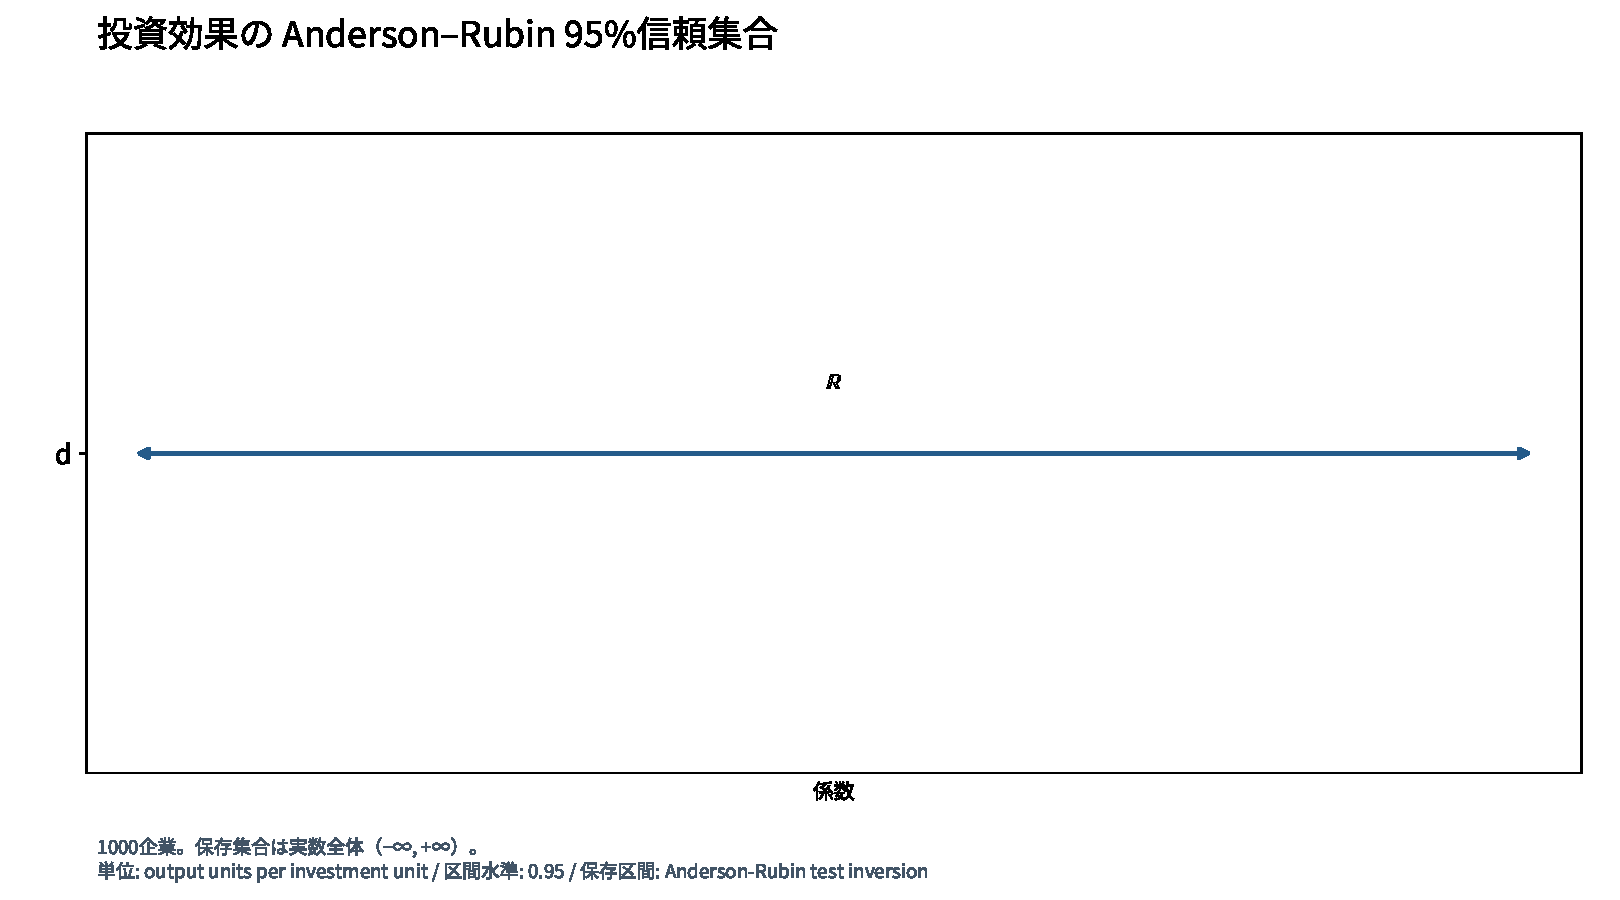
\includegraphics[keepaspectratio,alt={投資効果の Anderson--Rubin 95\%信頼集合}]{assets/exhibit-4-4.pdf}}

}

\caption{投資効果の Anderson--Rubin 95\%信頼集合.
1000企業。保存集合は実数全体（−∞, +∞）。標本: id\_column: id,
included\_rows: 1000, observations: 1000、母集団: 1000 simulated
firms、期間: one simulated choice occasion、単位: output units per
investment unit、推定対象: Anderson-Rubin confidence set for the linear
structural investment coefficient、推定方法: ivDiag::AR\_test、信頼区間:
0.95、N: 1000、推論: type: official、重み: 、区間の種類: Anderson-Rubin
test inversion、推論単位: id。結果ID:
specialist-weak-iv-r01。specialist-weak-iv-r01 生成元: model:
iv\_ar\_robust, specification: 8eab05628657}

\end{figure}%

\begin{minipage}{\linewidth}

\section{資格の閾値における局所効果}\label{result-5}

資格スコアが0以上の申請者を処置する制度について、閾値での成果の不連続を求める。対象は独立した1,600申請者の合成データである。潜在成果の条件付き平均の連続性と、スコアによる決定的な処置割当を採用する。rdrobust::rdrobust
に局所線形 p=1、バイアス補正
q=2、三角カーネル、MSE帯域選択、最近傍分散推定、信頼水準90\%を指定した。

\href{https://github.com/yoshimurahiroki/econ-project-mini/blob/f9093ba87cabce7bee1fdf3391656544617a8cb9/examples/research-workspace/models/rdd-spec.json}{入力仕様}・\href{https://github.com/yoshimurahiroki/econ-project-mini/blob/f9093ba87cabce7bee1fdf3391656544617a8cb9/examples/research-workspace/models/rdd-result.json}{計算結果}。

\begin{longtable}[]{@{}ll@{}}
\caption{括弧内は保存された標準誤差。単位: outcome units / 区間水準: 0.9
/ 保存区間: pointwise。標本: id\_column: id, observations: 1600、母集団:
1600 simulated applicants near the eligibility cutoff、期間: one
simulated choice occasion、単位: outcome units、推定対象: outcome
discontinuity at score zero、推定方法: rdrobust::rdrobust、信頼区間:
0.9、N: 1600、推論: type: official、重み: 、区間の種類:
pointwise。結果ID: specialist-rdd-r01。specialist-rdd-r01 生成元: model:
rdrobust\_r, specification: 2f4c144f291d}\tabularnewline
\toprule\noalign{}
項目 & 保存推定値 \\
\midrule\noalign{}
\endfirsthead
\toprule\noalign{}
項目 & 保存推定値 \\
\midrule\noalign{}
\endhead
\bottomrule\noalign{}
\endlastfoot
& (1) \\
閾値の効果 & 1.9059 \\
& (0.1076) \\
区間 & {[}1.7290, 2.0828{]} \\
p 値 & 2.9e-70 \\
観測数 & 1600 \\
統制変数 & \\
単位 & outcome units \\
\end{longtable}

\end{minipage}

\section{資格の閾値における局所効果の結果}\label{result-6}

バイアス補正後の局所効果は 1.905903、頑健標準誤差は 0.107552、90\%区間は
{[}1.728995, 2.082811{]}
である。推定帯域は左右とも0.285551、有効標本は左245人・右252人である。図は
rdplot
が保存した81区間平均と左右の2次曲線1,000座標を示す。図示帯域は左0.999028、右0.998783である。

\begin{figure}[H]

{\centering \pandocbounded{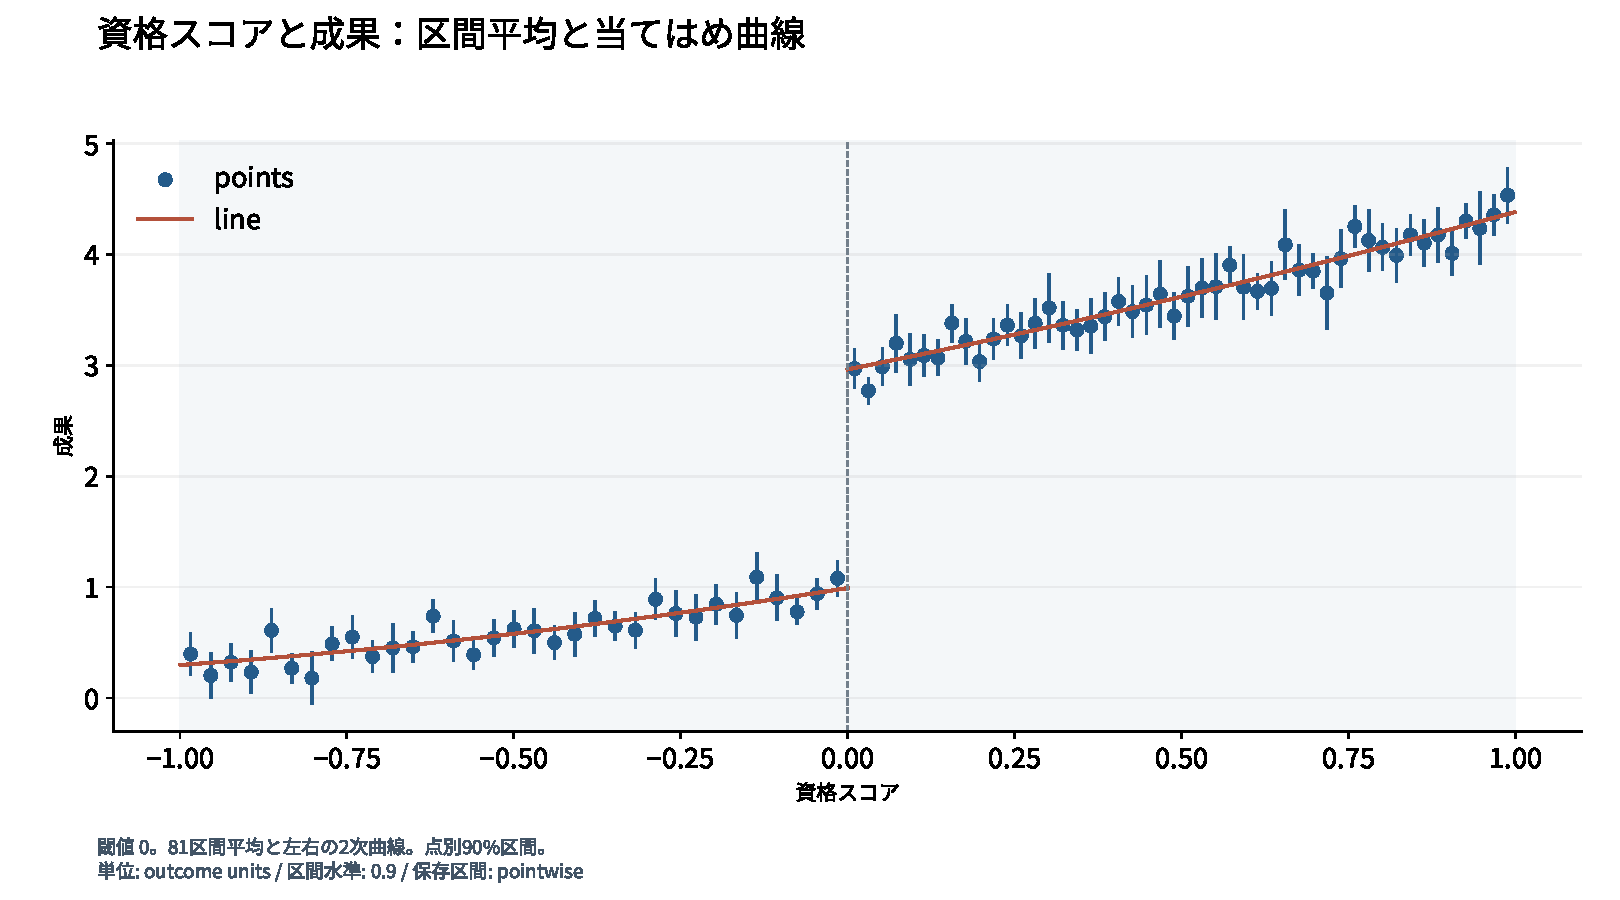
\includegraphics[keepaspectratio,alt={資格スコアと成果：区間平均と当てはめ曲線}]{assets/exhibit-6-4.pdf}}

}

\caption{資格スコアと成果：区間平均と当てはめ曲線. 閾値
0。81区間平均と左右の2次曲線。点別90\%区間。標本:
included\_ids\_available: False, input\_rows: 1600, observations:
1600、母集団: 1600 simulated applicants near the eligibility
cutoff、期間: one simulated choice occasion、単位: outcome
units、推定対象: Binned outcome means and left/right polynomial
conditional means、推定方法: rdrobust::rdrobust、信頼区間: 0.9、N:
1600、推論: type: official、重み: 、区間の種類: pointwise、cutoff:
0、bandwidth: 0.99902840687904, 0.9987830162091345。結果ID:
specialist-rdd-r01。specialist-rdd-r01 生成元: model: rdrobust\_r,
specification: 2f4c144f291d}

\end{figure}%

\begin{minipage}{\linewidth}

\section{所有統合による価格と厚生の変化}\label{result-7}

消費者は4製品か外部選択肢を選び、企業は所有製品の利潤を最大化する価格を選ぶ。120市場・480製品観測の合成データに、平均効用
1+prices+x と限界費用 1+z を指定し、需要・供給の操作変数を用いる1段階
GMM
で5母数を推定した。比較する介入は企業0と1の所有統合である。推定需要、各製品の推定限界費用、製品集合を固定する。統合企業は製品0・1の利潤を合わせて価格を決める。表の標準誤差は
PyBLP の保存値である。

\href{https://github.com/yoshimurahiroki/econ-project-mini/blob/f9093ba87cabce7bee1fdf3391656544617a8cb9/examples/research-workspace/models/blp-supply-spec.json}{入力仕様}・\href{https://github.com/yoshimurahiroki/econ-project-mini/blob/f9093ba87cabce7bee1fdf3391656544617a8cb9/examples/research-workspace/models/blp-supply-result.json}{計算結果}。

\begin{longtable}[]{@{}llll@{}}
\caption{単位: see row-specific unit、推論: Official ProblemResults
standard errors; fixed parameters retain their saved values、モデル契約:
MC-pyblp-bertrand。結果ID:
specialist-blp-supply-r01。specialist-blp-supply-r01 生成元: model: blp,
specification: 3f5761bc470f}\tabularnewline
\toprule\noalign{}
パラメータ & 値 & 標準誤差 & 単位 \\
\midrule\noalign{}
\endfirsthead
\toprule\noalign{}
パラメータ & 値 & 標準誤差 & 単位 \\
\midrule\noalign{}
\endhead
\bottomrule\noalign{}
\endlastfoot
beta{[}1{]} & 1.0587 & 0.0208 & utility per regressor unit \\
beta{[}prices{]} & -1.1247 & 0.0089 & utility per regressor unit \\
beta{[}x{]} & 0.5020 & 0.0017 & utility per regressor unit \\
gamma{[}1{]} & 1.3217 & 0.0080 & cost per regressor unit \\
gamma{[}z{]} & 0.3050 & 0.0026 & cost per regressor unit \\
\end{longtable}

\end{minipage}

\section{所有統合による価格と厚生の変化の結果}\label{result-8}

市場0の製品0の価格は2.141261から2.216112へ上昇する。潜在消費者1人当たりの消費者余剰は
0.550028 から 0.538838、生産者余剰は 0.471959 から 0.476527
となる。総余剰は 1.021988 から 1.015365
へ変化する。図は市場0--2の市場別の水準を示す。保存診断の GMM
勾配ノルムは 3.9e-10、利潤の価格勾配の最大絶対値は 7.52e-14 である。

\begin{figure}[H]

{\centering \pandocbounded{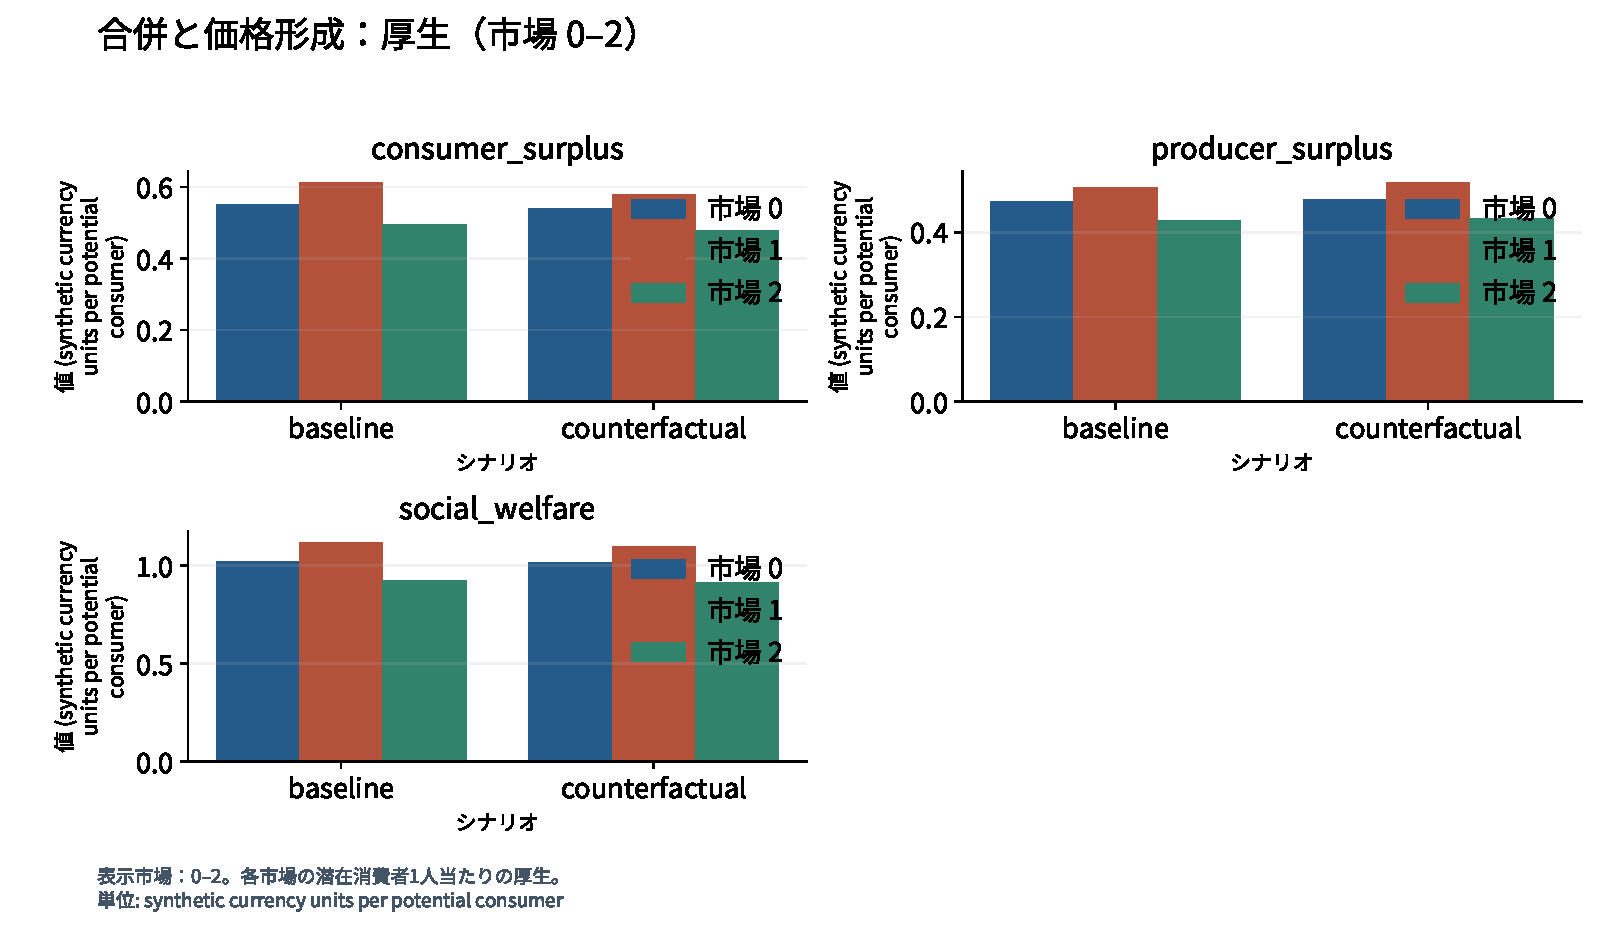
\includegraphics[keepaspectratio,alt={合併と価格形成：厚生（市場 0--2）}]{assets/exhibit-8-4.pdf}}

}

\caption{合併と価格形成：厚生（市場 0--2）.
表示市場：0--2。各市場の潜在消費者1人当たりの厚生。母集団: Potential
consumers within each market、単位: synthetic currency units per
potential consumer、モデル契約: MC-pyblp-bertrand。結果ID:
specialist-blp-supply-r01。specialist-blp-supply-r01 生成元: model: blp,
specification: 3f5761bc470f}

\end{figure}%

\begin{minipage}{\linewidth}

\section{固定した異質性と推定する平均係数}\label{result-9}

12市場・各3製品の合成データに、ランダム係数需要を当てはめる。平均効用は
1+prices+x、異質性を持つ項は 1+prices である。ランダム係数の Cholesky
因子の3要素を0.2・0.05・0.1に固定し、平均効用の3係数を GMM
で推定した。PyBLP の積型積分 size=5
を採用する。表は推定係数とその保存標準誤差、固定した異質性係数を示す。市場0の製品シェアを図に示す。

\href{https://github.com/yoshimurahiroki/econ-project-mini/blob/f9093ba87cabce7bee1fdf3391656544617a8cb9/examples/research-workspace/models/blp-fixed-spec.json}{入力仕様}・\href{https://github.com/yoshimurahiroki/econ-project-mini/blob/f9093ba87cabce7bee1fdf3391656544617a8cb9/examples/research-workspace/models/blp-fixed-result.json}{計算結果}。

\begin{longtable}[]{@{}
  >{\raggedright\arraybackslash}p{(\linewidth - 8\tabcolsep) * \real{0.2000}}
  >{\raggedright\arraybackslash}p{(\linewidth - 8\tabcolsep) * \real{0.2000}}
  >{\raggedright\arraybackslash}p{(\linewidth - 8\tabcolsep) * \real{0.2000}}
  >{\raggedright\arraybackslash}p{(\linewidth - 8\tabcolsep) * \real{0.2000}}
  >{\raggedright\arraybackslash}p{(\linewidth - 8\tabcolsep) * \real{0.2000}}@{}}
\caption{単位: see row-specific unit、推論: Official ProblemResults
bounds identify fixed parameters; standard errors retain the official
saved values、モデル契約: MC-pyblp-bertrand。結果ID:
specialist-blp-fixed-r01。specialist-blp-fixed-r01 生成元: model: blp,
specification: a22b03e4cd9d}\tabularnewline
\toprule\noalign{}
\begin{minipage}[b]{\linewidth}\raggedright
パラメータ
\end{minipage} & \begin{minipage}[b]{\linewidth}\raggedright
扱い
\end{minipage} & \begin{minipage}[b]{\linewidth}\raggedright
値
\end{minipage} & \begin{minipage}[b]{\linewidth}\raggedright
標準誤差
\end{minipage} & \begin{minipage}[b]{\linewidth}\raggedright
単位
\end{minipage} \\
\midrule\noalign{}
\endfirsthead
\toprule\noalign{}
\begin{minipage}[b]{\linewidth}\raggedright
パラメータ
\end{minipage} & \begin{minipage}[b]{\linewidth}\raggedright
扱い
\end{minipage} & \begin{minipage}[b]{\linewidth}\raggedright
値
\end{minipage} & \begin{minipage}[b]{\linewidth}\raggedright
標準誤差
\end{minipage} & \begin{minipage}[b]{\linewidth}\raggedright
単位
\end{minipage} \\
\midrule\noalign{}
\endhead
\bottomrule\noalign{}
\endlastfoot
beta{[}1{]} & estimated & 0.9836 & 0.0480 & utility per regressor
unit \\
beta{[}prices{]} & estimated & -0.9981 & 0.0189 & utility per regressor
unit \\
beta{[}x{]} & estimated & 0.4037 & 0.0057 & utility per regressor
unit \\
sigma{[}1, 1{]} & fixed & 0.2000 & --- & utility per regressor unit \\
sigma{[}prices, 1{]} & fixed & 0.0500 & --- & utility per regressor
unit \\
sigma{[}prices, prices{]} & fixed & 0.1000 & --- & utility per regressor
unit \\
\end{longtable}

\end{minipage}

\section{固定した異質性と推定する平均係数の結果}\label{result-10}

価格係数は
−0.998107、標準誤差は0.018909である。市場0の製品0・1・2のシェアは0.102363・0.140231・0.168351となる。保存された
GMM 目的関数は 0.011881、観測シェアとの最大絶対差は 5.55e-17
である。異質性係数の固定値と平均係数の推定値を合わせて、この需要系を定義する。

\begin{figure}[H]

{\centering \pandocbounded{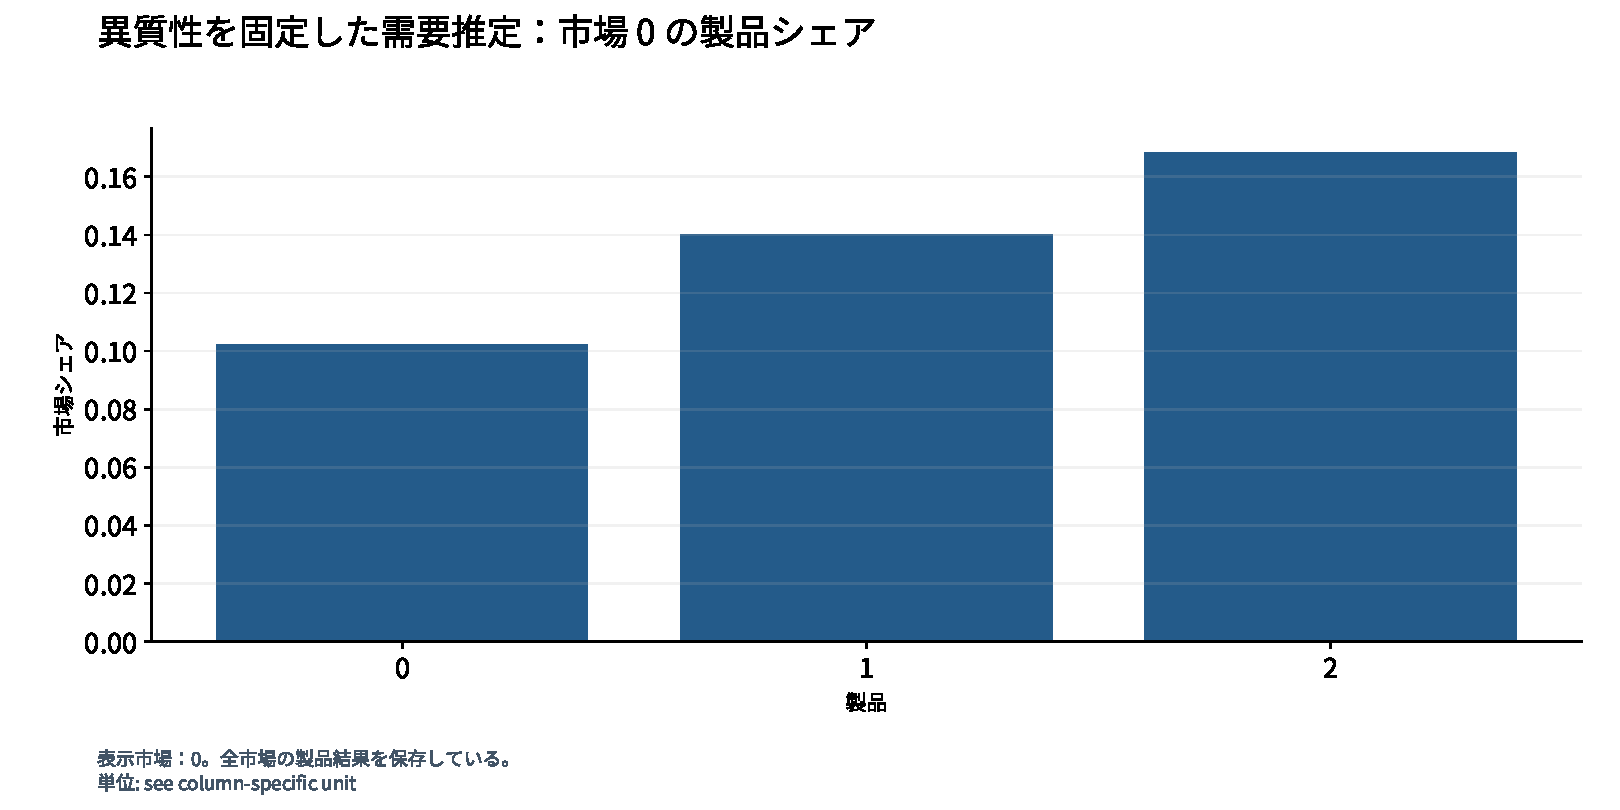
\includegraphics[keepaspectratio,alt={異質性を固定した需要推定：市場 0 の製品シェア}]{assets/exhibit-10-4.pdf}}

}

\caption{異質性を固定した需要推定：市場 0 の製品シェア.
表示市場：0。全市場の製品結果を保存している。単位: see column-specific
unit、モデル契約: MC-pyblp-bertrand。結果ID:
specialist-blp-fixed-r01。specialist-blp-fixed-r01 生成元: model: blp,
specification: a22b03e4cd9d}

\end{figure}%

\begin{minipage}{\linewidth}

\section{更新費用と状態別の行動}\label{result-11}

運行主体が走行距離状態を観察し、維持と更新を選ぶ。合成パネルは250主体・10,000観測、状態は5点、割引因子は0.9である。観測した状態・行動・次状態から遷移を推定し、ruspy
の NFXP 最尤法と同じ費用定義の CCP
推定を比較した。維持費用は走行距離状態に比例し、更新には固定費用を払う。比較状態では更新費用を0.5効用単位増やす。EV1ショックの尺度は1、Euler定数の正規化は0である。

\href{https://github.com/yoshimurahiroki/econ-project-mini/blob/f9093ba87cabce7bee1fdf3391656544617a8cb9/examples/research-workspace/models/replacement-spec.json}{入力仕様}・\href{https://github.com/yoshimurahiroki/econ-project-mini/blob/f9093ba87cabce7bee1fdf3391656544617a8cb9/examples/research-workspace/models/replacement-result.json}{計算結果}。

\begin{longtable}[]{@{}llll@{}}
\caption{単位: see row-specific unit、モデル契約:
MC-replacement-ddc、シナリオ: description: replacement cost rises by 0.5
utility units。結果ID: specialist-ddc-r01。specialist-ddc-r01 生成元:
model: replacement, specification: ea59473b0362}\tabularnewline
\toprule\noalign{}
推定法 & パラメータ & 値 & 単位 \\
\midrule\noalign{}
\endfirsthead
\toprule\noalign{}
推定法 & パラメータ & 値 & 単位 \\
\midrule\noalign{}
\endhead
\bottomrule\noalign{}
\endlastfoot
nfxp & maintenance\_cost & 0.2574 & utility per mileage state \\
nfxp & replacement\_cost & 2.1042 & utility \\
ccp & maintenance\_cost & 0.2591 & utility per mileage state \\
ccp & replacement\_cost & 2.1059 & utility \\
\end{longtable}

\end{minipage}

\section{更新費用と状態別の行動の結果}\label{result-12}

NFXP の更新費用は 2.104201、CCP は 2.105925
を返した。更新費用が上がると、走行状態0の更新確率は0.154458から0.106191へ低下する。同じ初期状態の期待割引効用は−2.363660から−3.616894となる。公式尤度との差は
1.82e-12、基準状態の Bellman 残差は 8.83e-13、費用上昇後は 8.62e-13
である。

\begin{figure}[H]

{\centering \pandocbounded{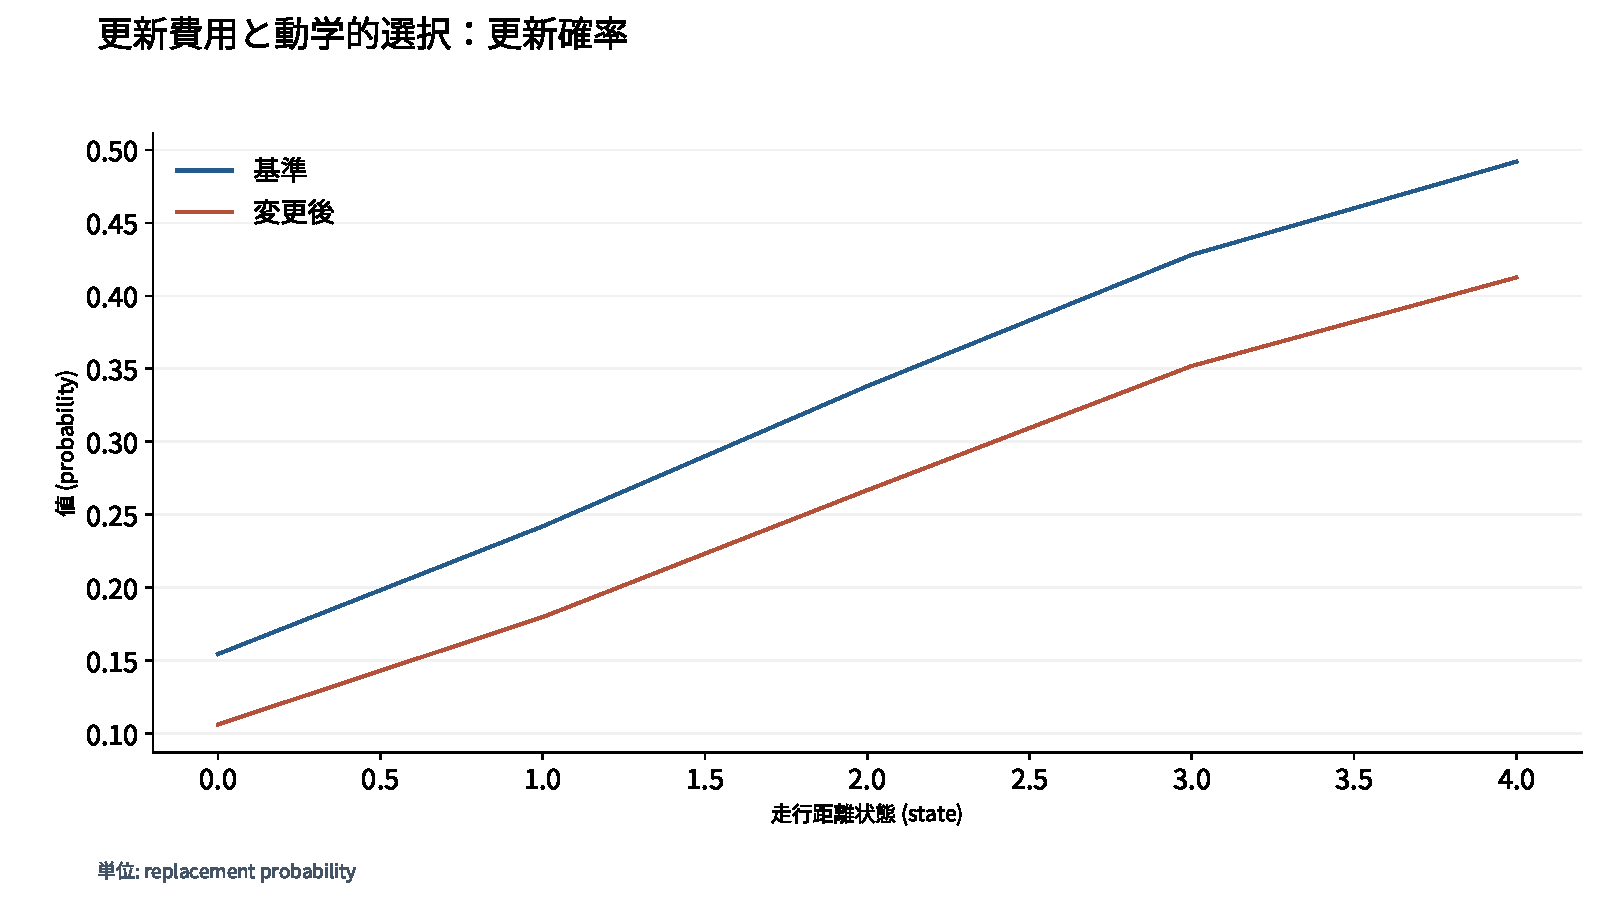
\includegraphics[keepaspectratio,alt={更新費用と動学的選択：更新確率}]{assets/exhibit-12-4.pdf}}

}

\caption{更新費用と動学的選択：更新確率. 単位: replacement
probability、推定対象: Optimal replacement probability conditional on
mileage state、モデル契約: MC-replacement-ddc、シナリオ: description:
replacement cost rises by 0.5 utility units。結果ID:
specialist-ddc-r01。specialist-ddc-r01 生成元: model: replacement,
specification: ea59473b0362}

\end{figure}%

\begin{minipage}{\linewidth}

\section{一時的な産出税と消費・資本}\label{result-13}

代表的家計が20期の割引対数効用を最大化する。資本弾力性0.33、割引因子0.96、減耗率0.08を較正し、初期・終端資本を4.4338357137に固定する。生産性は全期1である。基準状態の税率は0、比較状態は最初の10期が5\%、残り10期が0であり、税収は政府吸収に充てる。資源制約は
\(c_t+k_{t+1}=(1-\tau_t)A_t k_t^{\alpha}+(1-\delta)k_t\)。SciPy SLSQP
が正の消費と資本の経路を計算した。

\href{https://github.com/yoshimurahiroki/econ-project-mini/blob/f9093ba87cabce7bee1fdf3391656544617a8cb9/examples/research-workspace/models/growth-spec.json}{入力仕様}・\href{https://github.com/yoshimurahiroki/econ-project-mini/blob/f9093ba87cabce7bee1fdf3391656544617a8cb9/examples/research-workspace/models/growth-result.json}{計算結果}。

\begin{longtable}[]{@{}lll@{}}
\caption{母集団: one representative household、期間: 20 model
periods、単位: see row-specific unit、モデル契約:
MC-ramsey-cf、パラメータの扱い: specified、終端条件: fixed terminal
capital; no continuation utility。結果ID:
specialist-growth-r01。specialist-growth-r01 生成元: model:
finite-horizon deterministic household growth, specification:
6ab1f0c1cd1f}\tabularnewline
\toprule\noalign{}
パラメータ & 値 & 単位 \\
\midrule\noalign{}
\endfirsthead
\toprule\noalign{}
パラメータ & 値 & 単位 \\
\midrule\noalign{}
\endhead
\bottomrule\noalign{}
\endlastfoot
alpha & 0.3300 & capital elasticity \\
beta & 0.9600 & discount factor \\
delta & 0.0800 & depreciation rate \\
initial\_capital & 4.4338 & goods \\
terminal\_capital & 4.4338 & goods \\
\end{longtable}

\end{minipage}

\section{一時的な産出税と消費・資本の結果}\label{result-14}

期0の消費は1.279990から1.243608へ変化する。家計は課税期間に資本を取り崩し、終端に向けて資本を積み戻す。20期の割引対数効用は
3.443576 から 2.899971、保存された厚生差は -0.543605 である。変更後の
Euler 式の最大絶対残差は 3.14e-07、資源制約の残差は 0 で、採用許容値は
1e-5 である。

\begin{figure}[H]

{\centering \pandocbounded{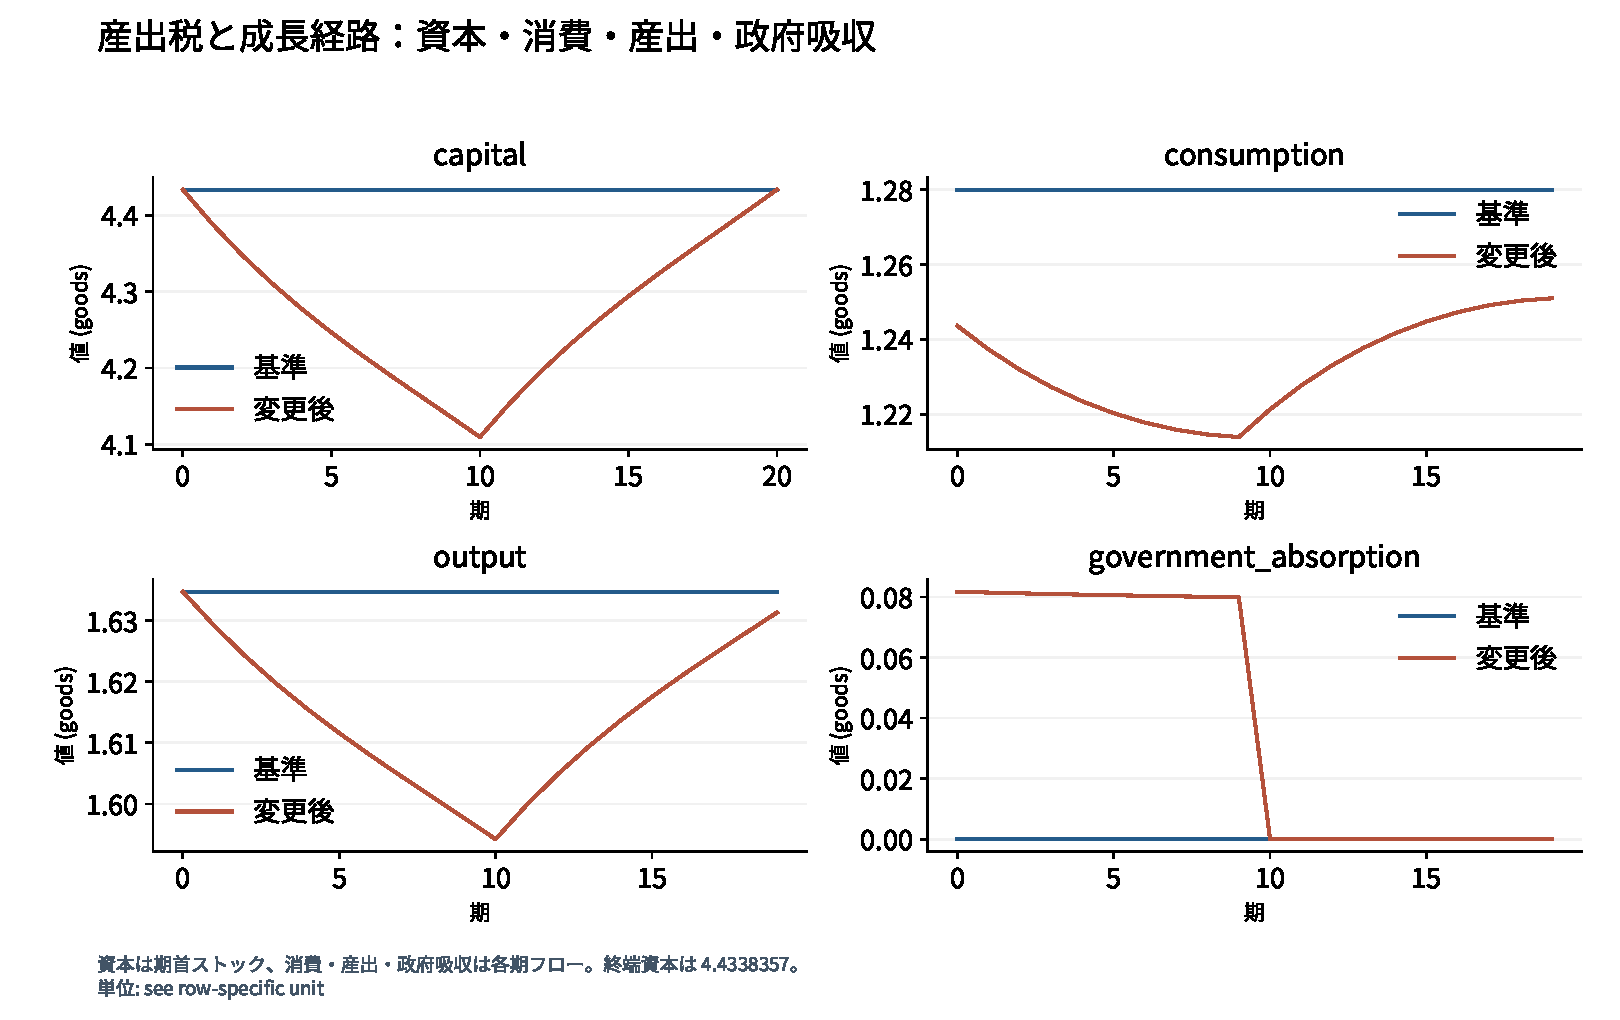
\includegraphics[keepaspectratio,alt={産出税と成長経路：資本・消費・産出・政府吸収}]{assets/exhibit-14-4.pdf}}

}

\caption{産出税と成長経路：資本・消費・産出・政府吸収.
資本は期首ストック、消費・産出・政府吸収は各期フロー。終端資本は
4.4338357。母集団: one representative household、期間: 20 model
periods、単位: see row-specific unit、モデル契約:
MC-ramsey-cf、終端条件: fixed terminal capital; no continuation
utility、時点の定義: Capital is the start-of-period stock, including the
terminal endpoint; other quantities are period flows。結果ID:
specialist-growth-r01。specialist-growth-r01 生成元: model:
finite-horizon deterministic household growth, specification:
6ab1f0c1cd1f}

\end{figure}%

\begin{minipage}{\linewidth}

\section{生産性と異質な家計の定常均衡}\label{result-15}

所得が変動する家計は、現在資産と所得を観察して消費と次期資産を選ぶ。資産は0--30の301点、労働効率は0.5と1.5、同じ所得状態に留まる確率は0.9である。資本弾力性0.36、割引因子0.96、減耗率0.08、相対的危険回避度2を較正した。QuantEcon
DiscreteDP
の政策反復と定常分布を用い、家計の資産供給と企業の資本需要を整合させる。比較する生産性は1と1.05である。各シナリオの定常分布で状態価値を平均し、定常均衡間の厚生を比較する。

\href{https://github.com/yoshimurahiroki/econ-project-mini/blob/f9093ba87cabce7bee1fdf3391656544617a8cb9/examples/research-workspace/models/aiyagari-spec.json}{入力仕様}・\href{https://github.com/yoshimurahiroki/econ-project-mini/blob/f9093ba87cabce7bee1fdf3391656544617a8cb9/examples/research-workspace/models/aiyagari-result.json}{計算結果}。

\begin{longtable}[]{@{}llll@{}}
\caption{表示項目：資本、消費、純利子率、賃金。各シナリオの定常均衡。母集団:
Unit mass of infinitely lived households、単位: see row-specific
unit、モデル契約: MC-aiyagari-stationary、シナリオ: productivity:
1.05、パラメータの扱い: calibrated。結果ID:
specialist-aiyagari-r01。specialist-aiyagari-r01 生成元: model:
aiyagari, specification: b8ce66ad0471}\tabularnewline
\toprule\noalign{}
シナリオ & 数量 & 値 & 単位 \\
\midrule\noalign{}
\endfirsthead
\toprule\noalign{}
シナリオ & 数量 & 値 & 単位 \\
\midrule\noalign{}
\endhead
\bottomrule\noalign{}
\endlastfoot
baseline & capital & 6.9402 & goods per household \\
baseline & consumption & 1.4535 & goods per household per period \\
baseline & interest\_rate & 0.0242 & net return per period \\
baseline & wage & 1.2855 & goods per efficiency unit of labor \\
scenario & capital & 7.4967 & goods per household \\
scenario & consumption & 1.5687 & goods per household per period \\
scenario & interest\_rate & 0.0241 & net return per period \\
scenario & wage & 1.3878 & goods per efficiency unit of labor \\
\end{longtable}

\end{minipage}

\section{生産性と異質な家計の定常均衡の結果}\label{result-16}

家計当たり資本は 6.940198 から 7.496708、各期消費は 1.453476 から
1.568680 へ増える。消費等価変分は基準消費の比率で 0.079544
となる。基準の資本市場残差は -0.003703、許容値は0.005である。両均衡の
Bellman
最大残差は1.07e-14、定常分布残差は1.73e-18となる。図は現在資産と所得状態ごとの次期資産を示す。

\begin{figure}[H]

{\centering \pandocbounded{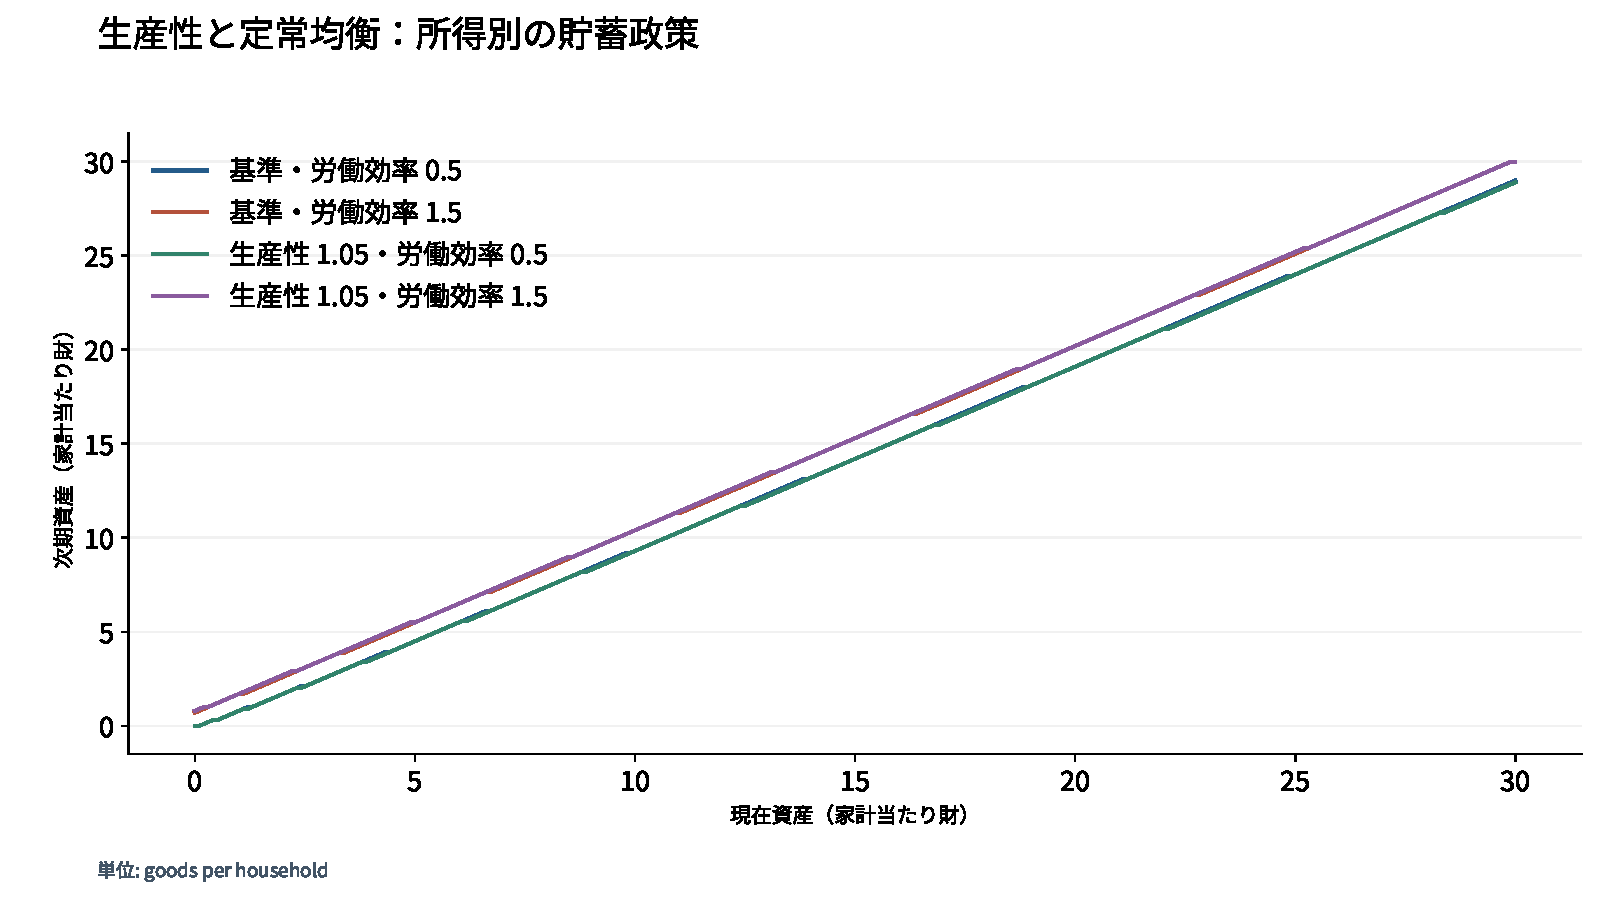
\includegraphics[keepaspectratio,alt={生産性と定常均衡：所得別の貯蓄政策}]{assets/exhibit-16-4.pdf}}

}

\caption{生産性と定常均衡：所得別の貯蓄政策. 母集団: Unit mass of
infinitely lived households、単位: goods per household、モデル契約:
MC-aiyagari-stationary、シナリオ: productivity: 1.05、パラメータの扱い:
calibrated。結果ID: specialist-aiyagari-r01。specialist-aiyagari-r01
生成元: model: aiyagari, specification: b8ce66ad0471}

\end{figure}%

%%%%%%%%%%%%%%%%%%%%%%%%%%%%%%%%%%%%%%%%%%%%%%
%% Single Appendix:            %%
%%%%%%%%%%%%%%%%%%%%%%%%%%%%%%%%%%%%%%%%%%%%%%
%\begin{appendix}
%\section*{???} %% if no title is needed, leave empty \section*{}.
%\end{appendix}
%%%%%%%%%%%%%%%%%%%%%%%%%%%%%%%%%%%%%%%%%%%%%%
%% Multiple Appendixes:        %%
%%%%%%%%%%%%%%%%%%%%%%%%%%%%%%%%%%%%%%%%%%%%%%
%\begin{appendix}
%\section{???}
%
%\section{???}
%\end{appendix}

%%%%%%%%%%%%%%%%%%%%%%%%%%%%%%%%%%%%%%%%%%%%%%
%% Bibliography:                            %%
%%%%%%%%%%%%%%%%%%%%%%%%%%%%%%%%%%%%%%%%%%%%%%
%% IMPORTANT: References in the bibliography should be complete,
%% including the first and last names, and date of publication.

%% If your bibliography is in bibtex format, uncomment commands:
% Bibliography style is set to ecta-fullname by the renderer.




\end{document}
